% Created by tikzDevice version 0.10.1 on 2018-01-24 12:52:03
% !TEX encoding = UTF-8 Unicode
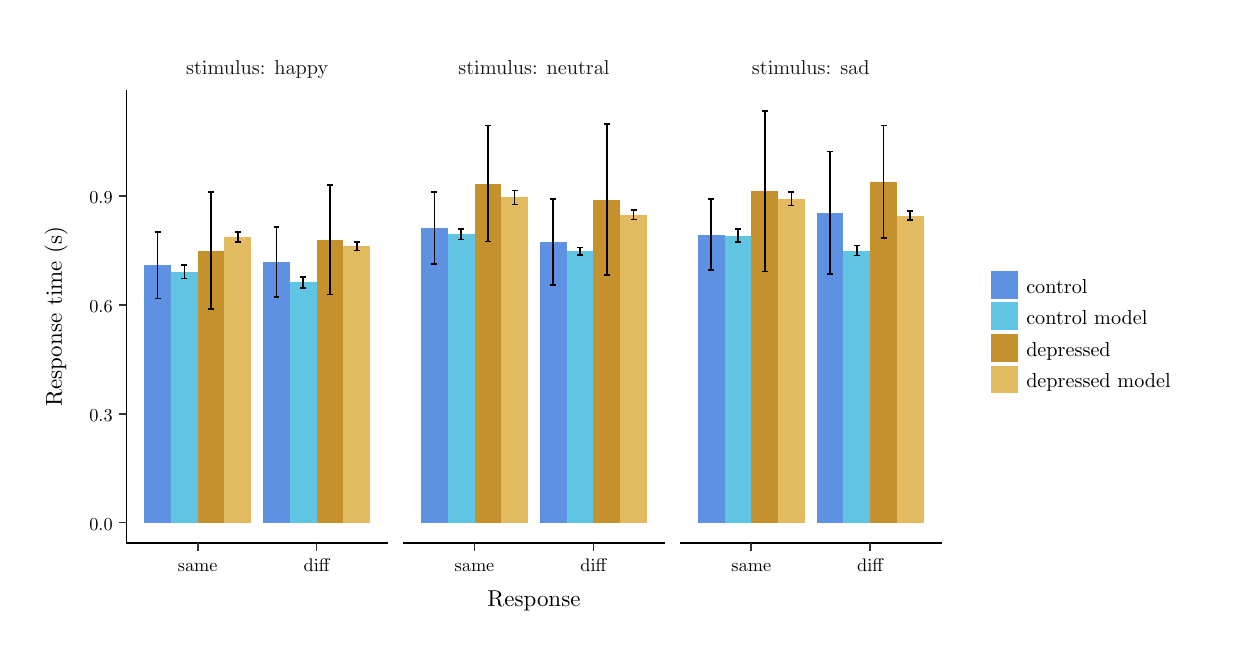
\begin{tikzpicture}[x=1pt,y=1pt]
\definecolor{fillColor}{RGB}{255,255,255}
\path[use as bounding box,fill=fillColor,fill opacity=0.00] (0,0) rectangle (433.62,216.81);
\begin{scope}
\path[clip] (  0.00,  0.00) rectangle (433.62,216.81);
\definecolor{drawColor}{RGB}{255,255,255}
\definecolor{fillColor}{RGB}{255,255,255}

\path[draw=drawColor,line width= 0.6pt,line join=round,line cap=round,fill=fillColor] (  0.00,  0.00) rectangle (433.62,216.81);
\end{scope}
\begin{scope}
\path[clip] ( 35.67, 30.56) rectangle (130.19,194.25);
\definecolor{fillColor}{RGB}{255,255,255}

\path[fill=fillColor] ( 35.67, 30.56) rectangle (130.19,194.25);
\definecolor{fillColor}{RGB}{226,186,95}

\path[fill=fillColor] ( 71.12, 38.00) rectangle ( 80.78,141.18);
\definecolor{fillColor}{RGB}{196,145,45}

\path[fill=fillColor] ( 61.45, 38.00) rectangle ( 71.12,136.24);
\definecolor{fillColor}{RGB}{95,197,226}

\path[fill=fillColor] ( 51.78, 38.00) rectangle ( 61.45,128.55);
\definecolor{fillColor}{RGB}{95,145,226}

\path[fill=fillColor] ( 42.12, 38.00) rectangle ( 51.78,131.00);
\definecolor{fillColor}{RGB}{226,186,95}

\path[fill=fillColor] (114.08, 38.00) rectangle (123.74,137.78);
\definecolor{fillColor}{RGB}{196,145,45}

\path[fill=fillColor] (104.41, 38.00) rectangle (114.08,140.17);
\definecolor{fillColor}{RGB}{95,197,226}

\path[fill=fillColor] ( 94.75, 38.00) rectangle (104.41,124.73);
\definecolor{fillColor}{RGB}{95,145,226}

\path[fill=fillColor] ( 85.08, 38.00) rectangle ( 94.75,132.18);
\definecolor{drawColor}{RGB}{0,0,0}

\path[draw=drawColor,line width= 0.6pt,line join=round] ( 74.88,142.99) --
	( 77.02,142.99);

\path[draw=drawColor,line width= 0.6pt,line join=round] ( 75.95,142.99) --
	( 75.95,139.37);

\path[draw=drawColor,line width= 0.6pt,line join=round] ( 74.88,139.37) --
	( 77.02,139.37);

\path[draw=drawColor,line width= 0.6pt,line join=round] ( 65.21,157.33) --
	( 67.36,157.33);

\path[draw=drawColor,line width= 0.6pt,line join=round] ( 66.28,157.33) --
	( 66.28,115.15);

\path[draw=drawColor,line width= 0.6pt,line join=round] ( 65.21,115.15) --
	( 67.36,115.15);

\path[draw=drawColor,line width= 0.6pt,line join=round] ( 55.54,130.96) --
	( 57.69,130.96);

\path[draw=drawColor,line width= 0.6pt,line join=round] ( 56.62,130.96) --
	( 56.62,126.15);

\path[draw=drawColor,line width= 0.6pt,line join=round] ( 55.54,126.15) --
	( 57.69,126.15);

\path[draw=drawColor,line width= 0.6pt,line join=round] ( 45.88,143.06) --
	( 48.03,143.06);

\path[draw=drawColor,line width= 0.6pt,line join=round] ( 46.95,143.06) --
	( 46.95,118.95);

\path[draw=drawColor,line width= 0.6pt,line join=round] ( 45.88,118.95) --
	( 48.03,118.95);

\path[draw=drawColor,line width= 0.6pt,line join=round] (117.84,139.26) --
	(119.99,139.26);

\path[draw=drawColor,line width= 0.6pt,line join=round] (118.91,139.26) --
	(118.91,136.31);

\path[draw=drawColor,line width= 0.6pt,line join=round] (117.84,136.31) --
	(119.99,136.31);

\path[draw=drawColor,line width= 0.6pt,line join=round] (108.17,159.95) --
	(110.32,159.95);

\path[draw=drawColor,line width= 0.6pt,line join=round] (109.24,159.95) --
	(109.24,120.39);

\path[draw=drawColor,line width= 0.6pt,line join=round] (108.17,120.39) --
	(110.32,120.39);

\path[draw=drawColor,line width= 0.6pt,line join=round] ( 98.50,126.66) --
	(100.65,126.66);

\path[draw=drawColor,line width= 0.6pt,line join=round] ( 99.58,126.66) --
	( 99.58,122.80);

\path[draw=drawColor,line width= 0.6pt,line join=round] ( 98.50,122.80) --
	(100.65,122.80);

\path[draw=drawColor,line width= 0.6pt,line join=round] ( 88.84,144.89) --
	( 90.99,144.89);

\path[draw=drawColor,line width= 0.6pt,line join=round] ( 89.91,144.89) --
	( 89.91,119.48);

\path[draw=drawColor,line width= 0.6pt,line join=round] ( 88.84,119.48) --
	( 90.99,119.48);
\end{scope}
\begin{scope}
\path[clip] (135.69, 30.56) rectangle (230.20,194.25);
\definecolor{fillColor}{RGB}{255,255,255}

\path[fill=fillColor] (135.69, 30.56) rectangle (230.20,194.25);
\definecolor{fillColor}{RGB}{226,186,95}

\path[fill=fillColor] (171.13, 38.00) rectangle (180.80,155.45);
\definecolor{fillColor}{RGB}{196,145,45}

\path[fill=fillColor] (161.47, 38.00) rectangle (171.13,160.48);
\definecolor{fillColor}{RGB}{95,197,226}

\path[fill=fillColor] (151.80, 38.00) rectangle (161.47,142.21);
\definecolor{fillColor}{RGB}{95,145,226}

\path[fill=fillColor] (142.13, 38.00) rectangle (151.80,144.50);
\definecolor{fillColor}{RGB}{226,186,95}

\path[fill=fillColor] (214.09, 38.00) rectangle (223.76,149.27);
\definecolor{fillColor}{RGB}{196,145,45}

\path[fill=fillColor] (204.43, 38.00) rectangle (214.09,154.71);
\definecolor{fillColor}{RGB}{95,197,226}

\path[fill=fillColor] (194.76, 38.00) rectangle (204.43,136.04);
\definecolor{fillColor}{RGB}{95,145,226}

\path[fill=fillColor] (185.09, 38.00) rectangle (194.76,139.39);
\definecolor{drawColor}{RGB}{0,0,0}

\path[draw=drawColor,line width= 0.6pt,line join=round] (174.89,158.01) --
	(177.04,158.01);

\path[draw=drawColor,line width= 0.6pt,line join=round] (175.96,158.01) --
	(175.96,152.89);

\path[draw=drawColor,line width= 0.6pt,line join=round] (174.89,152.89) --
	(177.04,152.89);

\path[draw=drawColor,line width= 0.6pt,line join=round] (165.22,181.44) --
	(167.37,181.44);

\path[draw=drawColor,line width= 0.6pt,line join=round] (166.30,181.44) --
	(166.30,139.52);

\path[draw=drawColor,line width= 0.6pt,line join=round] (165.22,139.52) --
	(167.37,139.52);

\path[draw=drawColor,line width= 0.6pt,line join=round] (155.56,144.15) --
	(157.71,144.15);

\path[draw=drawColor,line width= 0.6pt,line join=round] (156.63,144.15) --
	(156.63,140.27);

\path[draw=drawColor,line width= 0.6pt,line join=round] (155.56,140.27) --
	(157.71,140.27);

\path[draw=drawColor,line width= 0.6pt,line join=round] (145.89,157.47) --
	(148.04,157.47);

\path[draw=drawColor,line width= 0.6pt,line join=round] (146.97,157.47) --
	(146.97,131.53);

\path[draw=drawColor,line width= 0.6pt,line join=round] (145.89,131.53) --
	(148.04,131.53);

\path[draw=drawColor,line width= 0.6pt,line join=round] (217.85,151.04) --
	(220.00,151.04);

\path[draw=drawColor,line width= 0.6pt,line join=round] (218.93,151.04) --
	(218.93,147.49);

\path[draw=drawColor,line width= 0.6pt,line join=round] (217.85,147.49) --
	(220.00,147.49);

\path[draw=drawColor,line width= 0.6pt,line join=round] (208.19,181.96) --
	(210.33,181.96);

\path[draw=drawColor,line width= 0.6pt,line join=round] (209.26,181.96) --
	(209.26,127.47);

\path[draw=drawColor,line width= 0.6pt,line join=round] (208.19,127.47) --
	(210.33,127.47);

\path[draw=drawColor,line width= 0.6pt,line join=round] (198.52,137.37) --
	(200.67,137.37);

\path[draw=drawColor,line width= 0.6pt,line join=round] (199.59,137.37) --
	(199.59,134.72);

\path[draw=drawColor,line width= 0.6pt,line join=round] (198.52,134.72) --
	(200.67,134.72);

\path[draw=drawColor,line width= 0.6pt,line join=round] (188.85,154.85) --
	(191.00,154.85);

\path[draw=drawColor,line width= 0.6pt,line join=round] (189.93,154.85) --
	(189.93,123.93);

\path[draw=drawColor,line width= 0.6pt,line join=round] (188.85,123.93) --
	(191.00,123.93);
\end{scope}
\begin{scope}
\path[clip] (235.70, 30.56) rectangle (330.22,194.25);
\definecolor{fillColor}{RGB}{255,255,255}

\path[fill=fillColor] (235.70, 30.56) rectangle (330.22,194.25);
\definecolor{fillColor}{RGB}{226,186,95}

\path[fill=fillColor] (271.15, 38.00) rectangle (280.81,154.99);
\definecolor{fillColor}{RGB}{196,145,45}

\path[fill=fillColor] (261.48, 38.00) rectangle (271.15,157.73);
\definecolor{fillColor}{RGB}{95,197,226}

\path[fill=fillColor] (251.81, 38.00) rectangle (261.48,141.62);
\definecolor{fillColor}{RGB}{95,145,226}

\path[fill=fillColor] (242.15, 38.00) rectangle (251.81,142.01);
\definecolor{fillColor}{RGB}{226,186,95}

\path[fill=fillColor] (314.11, 38.00) rectangle (323.77,148.87);
\definecolor{fillColor}{RGB}{196,145,45}

\path[fill=fillColor] (304.44, 38.00) rectangle (314.11,161.13);
\definecolor{fillColor}{RGB}{95,197,226}

\path[fill=fillColor] (294.77, 38.00) rectangle (304.44,136.28);
\definecolor{fillColor}{RGB}{95,145,226}

\path[fill=fillColor] (285.11, 38.00) rectangle (294.77,149.87);
\definecolor{drawColor}{RGB}{0,0,0}

\path[draw=drawColor,line width= 0.6pt,line join=round] (274.90,157.39) --
	(277.05,157.39);

\path[draw=drawColor,line width= 0.6pt,line join=round] (275.98,157.39) --
	(275.98,152.60);

\path[draw=drawColor,line width= 0.6pt,line join=round] (274.90,152.60) --
	(277.05,152.60);

\path[draw=drawColor,line width= 0.6pt,line join=round] (265.24,186.81) --
	(267.39,186.81);

\path[draw=drawColor,line width= 0.6pt,line join=round] (266.31,186.81) --
	(266.31,128.65);

\path[draw=drawColor,line width= 0.6pt,line join=round] (265.24,128.65) --
	(267.39,128.65);

\path[draw=drawColor,line width= 0.6pt,line join=round] (255.57,143.98) --
	(257.72,143.98);

\path[draw=drawColor,line width= 0.6pt,line join=round] (256.65,143.98) --
	(256.65,139.26);

\path[draw=drawColor,line width= 0.6pt,line join=round] (255.57,139.26) --
	(257.72,139.26);

\path[draw=drawColor,line width= 0.6pt,line join=round] (245.91,154.85) --
	(248.05,154.85);

\path[draw=drawColor,line width= 0.6pt,line join=round] (246.98,154.85) --
	(246.98,129.17);

\path[draw=drawColor,line width= 0.6pt,line join=round] (245.91,129.17) --
	(248.05,129.17);

\path[draw=drawColor,line width= 0.6pt,line join=round] (317.87,150.50) --
	(320.01,150.50);

\path[draw=drawColor,line width= 0.6pt,line join=round] (318.94,150.50) --
	(318.94,147.23);

\path[draw=drawColor,line width= 0.6pt,line join=round] (317.87,147.23) --
	(320.01,147.23);

\path[draw=drawColor,line width= 0.6pt,line join=round] (308.20,181.44) --
	(310.35,181.44);

\path[draw=drawColor,line width= 0.6pt,line join=round] (309.27,181.44) --
	(309.27,140.83);

\path[draw=drawColor,line width= 0.6pt,line join=round] (308.20,140.83) --
	(310.35,140.83);

\path[draw=drawColor,line width= 0.6pt,line join=round] (298.53,138.05) --
	(300.68,138.05);

\path[draw=drawColor,line width= 0.6pt,line join=round] (299.61,138.05) --
	(299.61,134.52);

\path[draw=drawColor,line width= 0.6pt,line join=round] (298.53,134.52) --
	(300.68,134.52);

\path[draw=drawColor,line width= 0.6pt,line join=round] (288.87,172.01) --
	(291.01,172.01);

\path[draw=drawColor,line width= 0.6pt,line join=round] (289.94,172.01) --
	(289.94,127.73);

\path[draw=drawColor,line width= 0.6pt,line join=round] (288.87,127.73) --
	(291.01,127.73);
\end{scope}
\begin{scope}
\path[clip] ( 35.67,194.25) rectangle (130.19,211.31);
\definecolor{drawColor}{RGB}{255,255,255}
\definecolor{fillColor}{RGB}{255,255,255}

\path[draw=drawColor,line width= 1.1pt,line join=round,line cap=round,fill=fillColor] ( 35.67,194.25) rectangle (130.19,211.31);
\definecolor{drawColor}{gray}{0.10}

\node[text=drawColor,anchor=base,inner sep=0pt, outer sep=0pt, scale=  0.73] at ( 82.93,199.75) {stimulus: happy};
\end{scope}
\begin{scope}
\path[clip] (135.69,194.25) rectangle (230.20,211.31);
\definecolor{drawColor}{RGB}{255,255,255}
\definecolor{fillColor}{RGB}{255,255,255}

\path[draw=drawColor,line width= 1.1pt,line join=round,line cap=round,fill=fillColor] (135.69,194.25) rectangle (230.20,211.31);
\definecolor{drawColor}{gray}{0.10}

\node[text=drawColor,anchor=base,inner sep=0pt, outer sep=0pt, scale=  0.73] at (182.95,199.75) {stimulus: neutral};
\end{scope}
\begin{scope}
\path[clip] (235.70,194.25) rectangle (330.22,211.31);
\definecolor{drawColor}{RGB}{255,255,255}
\definecolor{fillColor}{RGB}{255,255,255}

\path[draw=drawColor,line width= 1.1pt,line join=round,line cap=round,fill=fillColor] (235.70,194.25) rectangle (330.22,211.31);
\definecolor{drawColor}{gray}{0.10}

\node[text=drawColor,anchor=base,inner sep=0pt, outer sep=0pt, scale=  0.73] at (282.96,199.75) {stimulus: sad};
\end{scope}
\begin{scope}
\path[clip] (  0.00,  0.00) rectangle (433.62,216.81);
\definecolor{drawColor}{RGB}{0,0,0}

\path[draw=drawColor,line width= 0.6pt,line join=round] ( 35.67, 30.56) --
	(130.19, 30.56);
\end{scope}
\begin{scope}
\path[clip] (  0.00,  0.00) rectangle (433.62,216.81);
\definecolor{drawColor}{gray}{0.20}

\path[draw=drawColor,line width= 0.6pt,line join=round] ( 61.45, 27.81) --
	( 61.45, 30.56);

\path[draw=drawColor,line width= 0.6pt,line join=round] (104.41, 27.81) --
	(104.41, 30.56);
\end{scope}
\begin{scope}
\path[clip] (  0.00,  0.00) rectangle (433.62,216.81);
\definecolor{drawColor}{RGB}{0,0,0}

\node[text=drawColor,anchor=base,inner sep=0pt, outer sep=0pt, scale=  0.66] at ( 61.45, 20.15) {same};

\node[text=drawColor,anchor=base,inner sep=0pt, outer sep=0pt, scale=  0.66] at (104.41, 20.15) {diff};
\end{scope}
\begin{scope}
\path[clip] (  0.00,  0.00) rectangle (433.62,216.81);
\definecolor{drawColor}{RGB}{0,0,0}

\path[draw=drawColor,line width= 0.6pt,line join=round] (135.69, 30.56) --
	(230.20, 30.56);
\end{scope}
\begin{scope}
\path[clip] (  0.00,  0.00) rectangle (433.62,216.81);
\definecolor{drawColor}{gray}{0.20}

\path[draw=drawColor,line width= 0.6pt,line join=round] (161.47, 27.81) --
	(161.47, 30.56);

\path[draw=drawColor,line width= 0.6pt,line join=round] (204.43, 27.81) --
	(204.43, 30.56);
\end{scope}
\begin{scope}
\path[clip] (  0.00,  0.00) rectangle (433.62,216.81);
\definecolor{drawColor}{RGB}{0,0,0}

\node[text=drawColor,anchor=base,inner sep=0pt, outer sep=0pt, scale=  0.66] at (161.47, 20.15) {same};

\node[text=drawColor,anchor=base,inner sep=0pt, outer sep=0pt, scale=  0.66] at (204.43, 20.15) {diff};
\end{scope}
\begin{scope}
\path[clip] (  0.00,  0.00) rectangle (433.62,216.81);
\definecolor{drawColor}{RGB}{0,0,0}

\path[draw=drawColor,line width= 0.6pt,line join=round] (235.70, 30.56) --
	(330.22, 30.56);
\end{scope}
\begin{scope}
\path[clip] (  0.00,  0.00) rectangle (433.62,216.81);
\definecolor{drawColor}{gray}{0.20}

\path[draw=drawColor,line width= 0.6pt,line join=round] (261.48, 27.81) --
	(261.48, 30.56);

\path[draw=drawColor,line width= 0.6pt,line join=round] (304.44, 27.81) --
	(304.44, 30.56);
\end{scope}
\begin{scope}
\path[clip] (  0.00,  0.00) rectangle (433.62,216.81);
\definecolor{drawColor}{RGB}{0,0,0}

\node[text=drawColor,anchor=base,inner sep=0pt, outer sep=0pt, scale=  0.66] at (261.48, 20.15) {same};

\node[text=drawColor,anchor=base,inner sep=0pt, outer sep=0pt, scale=  0.66] at (304.44, 20.15) {diff};
\end{scope}
\begin{scope}
\path[clip] (  0.00,  0.00) rectangle (433.62,216.81);
\definecolor{drawColor}{RGB}{0,0,0}

\path[draw=drawColor,line width= 0.6pt,line join=round] ( 35.67, 30.56) --
	( 35.67,194.25);
\end{scope}
\begin{scope}
\path[clip] (  0.00,  0.00) rectangle (433.62,216.81);
\definecolor{drawColor}{RGB}{0,0,0}

\node[text=drawColor,anchor=base east,inner sep=0pt, outer sep=0pt, scale=  0.66] at ( 30.72, 35.27) {0.0};

\node[text=drawColor,anchor=base east,inner sep=0pt, outer sep=0pt, scale=  0.66] at ( 30.72, 74.57) {0.3};

\node[text=drawColor,anchor=base east,inner sep=0pt, outer sep=0pt, scale=  0.66] at ( 30.72,113.87) {0.6};

\node[text=drawColor,anchor=base east,inner sep=0pt, outer sep=0pt, scale=  0.66] at ( 30.72,153.17) {0.9};
\end{scope}
\begin{scope}
\path[clip] (  0.00,  0.00) rectangle (433.62,216.81);
\definecolor{drawColor}{gray}{0.20}

\path[draw=drawColor,line width= 0.6pt,line join=round] ( 32.92, 38.00) --
	( 35.67, 38.00);

\path[draw=drawColor,line width= 0.6pt,line join=round] ( 32.92, 77.30) --
	( 35.67, 77.30);

\path[draw=drawColor,line width= 0.6pt,line join=round] ( 32.92,116.59) --
	( 35.67,116.59);

\path[draw=drawColor,line width= 0.6pt,line join=round] ( 32.92,155.89) --
	( 35.67,155.89);
\end{scope}
\begin{scope}
\path[clip] (  0.00,  0.00) rectangle (433.62,216.81);
\definecolor{drawColor}{RGB}{0,0,0}

\node[text=drawColor,anchor=base,inner sep=0pt, outer sep=0pt, scale=  0.83] at (182.95,  7.83) {Response};
\end{scope}
\begin{scope}
\path[clip] (  0.00,  0.00) rectangle (433.62,216.81);
\definecolor{drawColor}{RGB}{0,0,0}

\node[text=drawColor,rotate= 90.00,anchor=base,inner sep=0pt, outer sep=0pt, scale=  0.83] at ( 12.32,112.40) {Response time (s)};
\end{scope}
\begin{scope}
\path[clip] (  0.00,  0.00) rectangle (433.62,216.81);
\definecolor{fillColor}{RGB}{255,255,255}

\path[fill=fillColor] (341.60, 78.37) rectangle (428.12,146.43);
\end{scope}
\begin{scope}
\path[clip] (  0.00,  0.00) rectangle (433.62,216.81);
\definecolor{fillColor}{RGB}{95,145,226}

\path[fill=fillColor] (348.00,118.92) rectangle (357.96,128.88);
\end{scope}
\begin{scope}
\path[clip] (  0.00,  0.00) rectangle (433.62,216.81);
\definecolor{fillColor}{RGB}{95,197,226}

\path[fill=fillColor] (348.00,107.54) rectangle (357.96,117.50);
\end{scope}
\begin{scope}
\path[clip] (  0.00,  0.00) rectangle (433.62,216.81);
\definecolor{fillColor}{RGB}{196,145,45}

\path[fill=fillColor] (348.00, 96.16) rectangle (357.96,106.11);
\end{scope}
\begin{scope}
\path[clip] (  0.00,  0.00) rectangle (433.62,216.81);
\definecolor{fillColor}{RGB}{226,186,95}

\path[fill=fillColor] (348.00, 84.77) rectangle (357.96, 94.73);
\end{scope}
\begin{scope}
\path[clip] (  0.00,  0.00) rectangle (433.62,216.81);
\definecolor{drawColor}{RGB}{0,0,0}

\node[text=drawColor,anchor=base west,inner sep=0pt, outer sep=0pt, scale=  0.73] at (360.84,120.87) {control};
\end{scope}
\begin{scope}
\path[clip] (  0.00,  0.00) rectangle (433.62,216.81);
\definecolor{drawColor}{RGB}{0,0,0}

\node[text=drawColor,anchor=base west,inner sep=0pt, outer sep=0pt, scale=  0.73] at (360.84,109.49) {control model};
\end{scope}
\begin{scope}
\path[clip] (  0.00,  0.00) rectangle (433.62,216.81);
\definecolor{drawColor}{RGB}{0,0,0}

\node[text=drawColor,anchor=base west,inner sep=0pt, outer sep=0pt, scale=  0.73] at (360.84, 98.10) {depressed};
\end{scope}
\begin{scope}
\path[clip] (  0.00,  0.00) rectangle (433.62,216.81);
\definecolor{drawColor}{RGB}{0,0,0}

\node[text=drawColor,anchor=base west,inner sep=0pt, outer sep=0pt, scale=  0.73] at (360.84, 86.72) {depressed model};
\end{scope}
\end{tikzpicture}
